\vspace{-1cm}\emph{\small We follow the standard derivation of \citet{Murphy12b}. This differs from that used by \cite{Murphy12}, who follow \citet{Murphy11} in using Lindblad's original approach. \citet{Murphy10} derive the approximation in heliocentric coordinates in terms of the initial $XYZ$ position and $UVW$ velocity of the test particle. The two derivations are equivalent, as are the standard angular frequencies $\Omega$, $\kappa$ and $\nu$.}\\

We first assume a gravitational potential for the Galactic disk $\Phi$ that is axisymmetric around the normal to the disk. We also assume that such a potential is symmetric about the disk plane. In cylindrical $(R,\phi,z)$ coordinates the equations of motion for such a potential are:
\begin{align}\label{eqn:eom}
\begin{split}
\ddot{R}-R\dot{\phi}^2& = -\frac{\partial \Phi}{\partial R} \\
\frac{d}{dt}(R^{2}\dot{\phi})& = 0 \\
\ddot{z}&=-\frac{\partial\Phi}{\partial z}
\end{split}
\end{align}
Noting that the second equation implies the conservation of angular momentum about the $z$ axis; $R^{2}\dot{\phi}=\textrm{constant} = L_{z}$, the equations of motion can also be written
\begin{align}\label{eqn:eqnmotion}
\begin{split}
\ddot{R} = -\frac{\partial \Phi_{\rm eff}}{\partial R} \quad\textrm{and}\quad \ddot{z} = -\frac{\partial \Phi_{\rm eff}}{\partial z} 
\end{split}
\end{align}
where the effective potential $\Phi_{\rm eff}(R,z)$ is defined as
\begin{align}
\Phi_{\rm eff}(R,z) = \Phi(R,z) + \frac{L_{z}^{2}}{2R^{2}}
\end{align}
The effective potential has a minimum at $z=0$ (by symmetry) and at $R=R_{g}$:
\begin{align}
\frac{\partial \Phi_{\rm eff}}{\partial R} = \frac{\partial \Phi}{\partial R} - \frac{L_{z}^{2}}{R^{3}} = 0 \quad\textrm{which means}\quad \frac{\partial \Phi}{\partial R}\bigg|_{(R_{g},0)} = \frac{L_{z}^{2}}{R_{g}^{3}} = R_{g}\dot{\phi}^{2}
\end{align}
The \emph{guiding centre} radius $R_{g}$ therefore corresponds to a circular orbit with constant angular speed $\dot{\phi}=\Omega_{g}=\sqrt{(1/R)\partial \Phi/\partial R}=L_{z}/R_{g}^{2}$. We can approximate the effective potential around $(R,z)=(R_{g},0)$ by the second-order Taylor expansion around this point. If we define $x=(R-R_{g})$ the expansion is:
\begin{align}
\begin{split}
\Phi_{\rm eff} &\simeq \Phi_{\rm eff}(R_{g},0) + x\frac{\partial\Phi_{\rm eff}}{\partial R}\bigg|_{(R_{g},0)} + z\frac{\partial\Phi_{\rm eff}}{\partial z}\bigg|_{(R_{g},0)}\\
&+ \frac{1}{2}x^{2}\frac{\partial^{2}\Phi_{\rm eff}}{\partial R^{2}}\bigg|_{(R_{g},0)} + \frac{1}{2}z^{2}\frac{\partial^{2}\Phi_{\rm eff}}{\partial z^{2}}\bigg|_{(R_{g},0)} + xz\frac{\partial^{2}\Phi_{\rm eff}}{\partial R\partial z}\bigg|_{(R_{g},0)} 
\end{split}
\end{align}
The second and third terms are zero at the point $(R_{g},0)$. The cross-term is also zero as we assume the potential is symmetric about $z=0$. The effective potential then becomes
\begin{align}
\begin{split}
\Phi_{\rm eff} &\simeq \Phi_{\rm eff}(R_{g},0) + \frac{1}{2}x^{2}\frac{\partial^{2}\Phi_{\rm eff}}{\partial R^{2}}\bigg|_{(R_{g},0)} + \frac{1}{2}z^{2}\frac{\partial^{2}\Phi_{\rm eff}}{\partial z^{2}}\bigg|_{(R_{g},0)}\\
&= \Phi_{\rm eff}(R_{g},0) + \frac{1}{2}(\kappa x)^{2} + \frac{1}{2}(\nu z)^{2}
\end{split}
\end{align}
where we define the constants:
\begin{align} 
\kappa^{2} = \frac{\partial^{2} \Phi_{\rm eff}}{\partial R^2}\bigg|_{(R_{g},0)} \quad\textrm{and}\quad \nu^{2} = \frac{\partial^{2} \Phi_{\rm eff}}{\partial z^2}\bigg|_{(R_{g},0)}
\end{align}
In this second-order Taylor expansion of the effective potential the equations of motion (Eqn. \ref{eqn:eqnmotion}) simplify to those of harmonic oscillators:
\begin{align}\label{eqn:harmonic}
\ddot{x} = -\kappa^{2} x \quad\textrm{and}\quad \ddot{z} = -\nu^{2} z
\end{align}
which have the general solutions:
\begin{align}\label{eqn:xz}
x(t) = X\cos(\kappa t + \alpha)\quad \textrm{and}\quad z(t) = Z\cos(\nu t + \beta)
\end{align}
for constants $X,Z,\alpha$ and $\beta$. What about the azimuthal coordinate $\phi$? Realising that angular momentum is conserved and $\dot{\phi}=L_{z}/R^{2}$ and $\Omega_{g}=L_{z}/R_{g}^{2}$, we have
\begin{align}
\dot{\phi} = \frac{L_{z}}{R_{g}^{2}}\frac{1}{(x/R_{g}+1)^{2}} \simeq \Omega_{g}\bigg(1-2\frac{x}{R_{g}}\bigg)
\end{align}
Substituting for $x(t)$ and integrating we arrive at
\begin{align}
\phi = \Omega_{g} t -2\frac{\Omega_{g}}{R_{g}\kappa}X\sin(\kappa t + \alpha) + \phi_{0}
\end{align}
If we convert the cylindrical $(R,\phi,z)$ coordinate system to a Cartesian system $(x,y,z)$, comoving with the guiding centre $(R_{g},\phi$); for $X \ll R_{g}$ this simplifies to:
\begin{align}
\begin{split}\label{eqn:y}
y(t) &= -2\frac{\Omega_{g}}{\kappa} X\sin(\kappa t + \alpha) \\
&= -Y\sin(\kappa t + \alpha)
\end{split}
\end{align}
In the new coordinate system $x$ and $z$ are the same as above and $y$ points in the direction of Galactic rotation. In this frame the star can  be thought of as simultaneously oscillating around the guiding centre vertically and in an ellipse in the $xy$ plane (the epicycle). The motion can be described by three angular frequencies; the epicyclic frequency $\kappa$, the vertical frequency $\nu$ and the angular velocity of the guiding centre, $\Omega_{g}$.  The vertical motion is independent of the epicyclic motion. The size of the epicycle is dictated by the ratio of $\kappa$ to $\Omega_{g}$: $X/Y = \kappa/2\Omega_{g}$.  The resultant orbital motion following Equations~\ref{eqn:xz} and \ref{eqn:y} in a Galactocentric inertial frame is traced in Figure~\ref{fig:orbit}. Like in the general case, although close to circular, the orbit is not closed in such a frame.

\begin{figure}[p!] 
\vspace{-2mm}
   \centering
   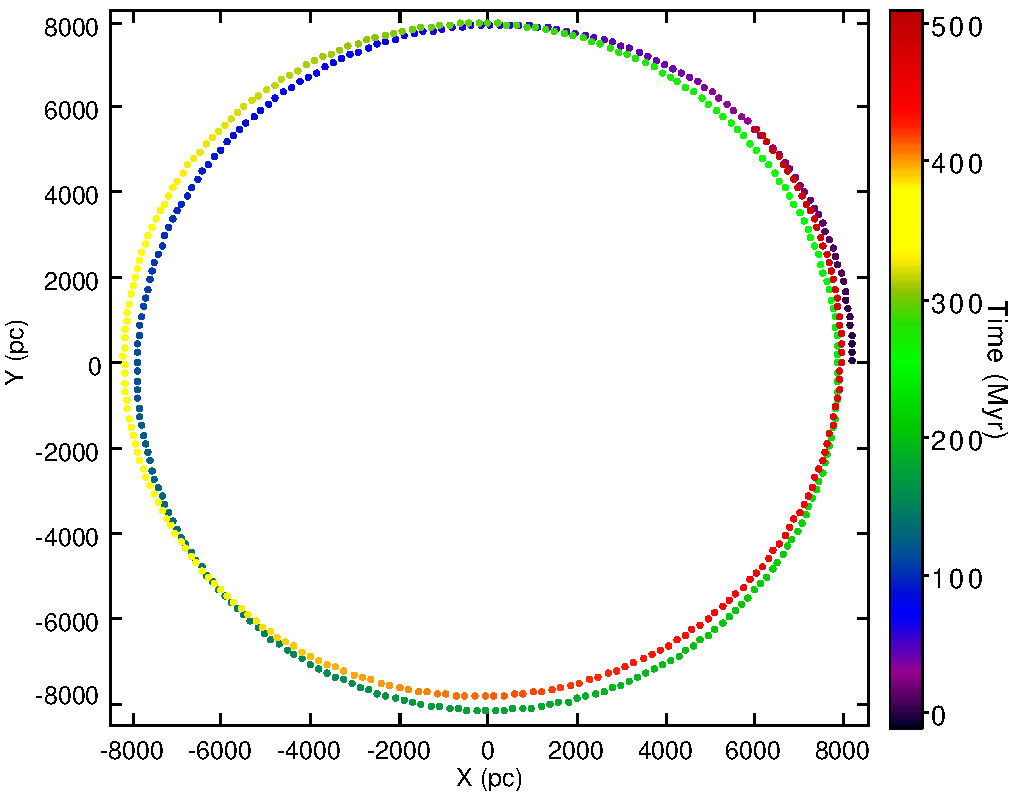
\includegraphics[width=0.68\textwidth]{orbit_xy}\\ 
   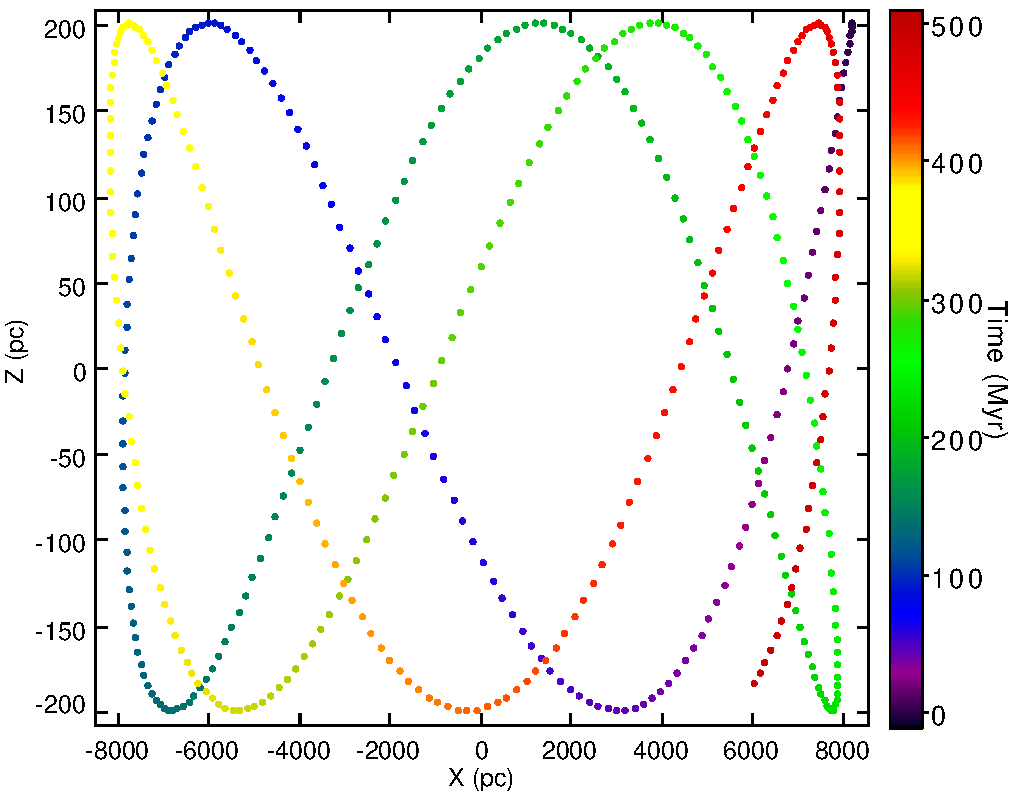
\includegraphics[width=0.68\textwidth]{orbit_xz}\\
   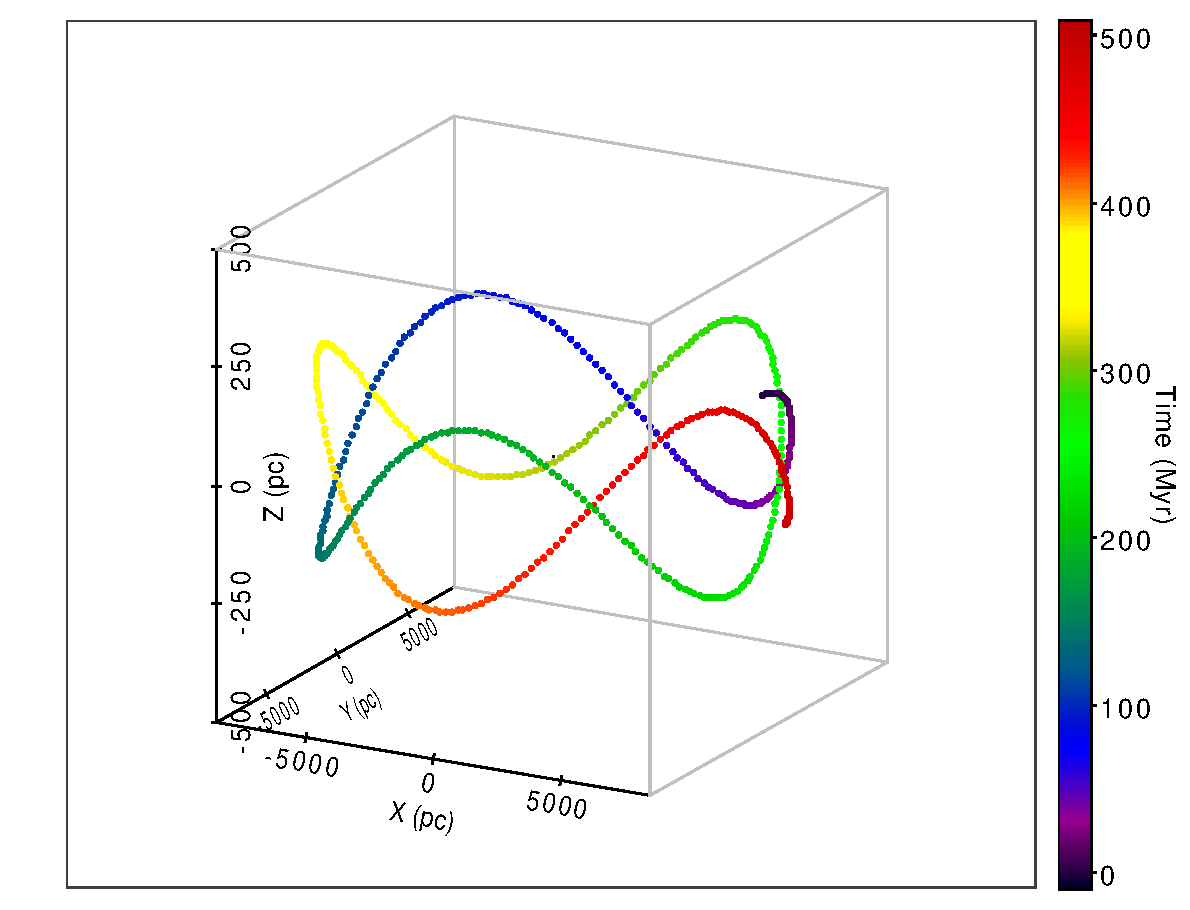
\includegraphics[width=0.68\textwidth]{orbit_xyz} 
   \caption[Orbital motion in the epicyclic approximation]{Orbital motion  with $\kappa_{0}=0.0367$~\kms~pc$^{-1}$ , $\Omega_{0}=0.0272$~\kms~pc$^{-1}$, $R_{g}=R_{\odot}=8000$~pc and $X=Z=200$~pc. The coordinate system has its origin at the Galactic centre.}
   \label{fig:orbit}
\end{figure}

